%==============================================================================
% On-Track-SysID for a full-scale Formula Student vehicle in CARLA
%
% Template: IEEEtran (journal), same class/bst as paper/My_master_thesis/.
% Build:  pdflatex main && bibtex main && pdflatex main && pdflatex main
%==============================================================================

\documentclass[journal]{IEEEtran}

\usepackage{xcolor}

\usepackage[pdftex]{graphicx}
\graphicspath{{figures/}{pdf/}{photo/}{../graphs/comparison/}}
\DeclareGraphicsExtensions{.pdf,.jpeg,.jpg,.png}

\usepackage[cmex10]{amsmath}
\usepackage{amssymb}
\usepackage{array}
\usepackage{multirow}
\usepackage{rotating}
\usepackage{eqparbox}
\usepackage{tabularx}
\usepackage{booktabs}
\usepackage{threeparttable}
\usepackage{url}
% --- lightweight algorithm float ---------------------------------------------
% float.sty ships with texlive-latex-recommended; the algorithm/algorithmicx
% families do not, so the body below is plain LaTeX rather than a new
% dependency.
\usepackage{float}
\newfloat{algorithm}{tbp}{loa}
\floatname{algorithm}{Algorithm}
\newcommand{\algline}[2]{\makebox[1.8em][r]{\scriptsize#1:}\ \ #2\par}
\newcommand{\algin}[1]{\hspace*{#1em}}
\usepackage{tikz}
\usetikzlibrary{positioning,arrows.meta,fit,backgrounds,calc}
% --- units -------------------------------------------------------------------
% Prefer siunitx (Debian/Ubuntu: it ships in texlive-science, NOT in
% texlive-latex-extra). If it is absent, fall back to units_fallback.tex, which
% implements exactly the macros used here. The branches must not be arguments
% to \IfFileExists -- a '#' inside such an argument is illegal -- hence the flag.
\newif\ifhavesiunitx
\IfFileExists{siunitx.sty}{\havesiunitxtrue}{\havesiunitxfalse}
\ifhavesiunitx
  \usepackage{siunitx}
  \sisetup{detect-all, per-mode=symbol}
  \DeclareSIUnit{\g}{\textit{g}}% g-force is not a predefined siunitx unit
\else
  % =============================================================================
% Minimal siunitx replacement.
%
% Loaded by main.tex ONLY when siunitx.sty is unavailable (on Debian/Ubuntu
% siunitx ships in texlive-science, not texlive-latex-extra). It implements
% exactly the macros this paper uses: \SI, \si, \num, \SIrange, \numrange and
% the unit names \meter \second \gram \newton \radian \hertz \percent \degree
% \g \kilo \milli \per \squared.
%
% All macros are declared robust: table captions are moving arguments
% (written to the .lot file), and an expandable conditional breaks there.
% Output matches siunitx closely; the one visible difference is that
% \SIrange/\numrange print an en-dash here where siunitx prints " to ".
% Install texlive-science to get the real package.
% =============================================================================

\makeatletter

% Separator state. Armed (true) once a base unit has been emitted; disarmed
% after a prefix and after \per, so "kilo newton per radian" sets no space
% between k and N, nor around the solidus.
\newif\ifsiu@prev
\DeclareRobustCommand{\siu@sep}{\ifsiu@prev\,\fi}
% \text{} (amsmath) so a unit typesets upright in BOTH text and math mode --
% these macros are routinely used inside $...$, where a bare `m` would come out
% as an italic math variable and `--` as two minus signs.
\DeclareRobustCommand{\siu@unit}[1]{\siu@sep\text{#1}\siu@prevtrue}  % base unit
\DeclareRobustCommand{\siu@pre}[1]{\siu@sep\text{#1}\siu@prevfalse}  % SI prefix
\DeclareRobustCommand{\siu@div}[1]{\text{#1}\siu@prevfalse}          % solidus

% Default (outside \si) meanings, so the unit names are always defined and
% \renewcommand below always has a target.
\DeclareRobustCommand{\meter}{m}
\DeclareRobustCommand{\second}{s}
\DeclareRobustCommand{\gram}{g}
\DeclareRobustCommand{\newton}{N}
\DeclareRobustCommand{\radian}{rad}
\DeclareRobustCommand{\hertz}{Hz}
\DeclareRobustCommand{\percent}{\%}
\DeclareRobustCommand{\g}{\textit{g}}
\DeclareRobustCommand{\kilo}{k}
\DeclareRobustCommand{\milli}{m}
\DeclareRobustCommand{\per}{/}
\DeclareRobustCommand{\squared}{\ensuremath{^{2}}}
\providecommand{\degree}{\ensuremath{^{\circ}}}

\DeclareRobustCommand{\si}[1]{\begingroup
  \siu@prevfalse
  \renewcommand{\meter}{\siu@unit{m}}%
  \renewcommand{\second}{\siu@unit{s}}%
  \renewcommand{\gram}{\siu@unit{g}}%
  \renewcommand{\newton}{\siu@unit{N}}%
  \renewcommand{\radian}{\siu@unit{rad}}%
  \renewcommand{\hertz}{\siu@unit{Hz}}%
  \renewcommand{\percent}{\siu@unit{\%}}%
  \renewcommand{\degree}{\siu@unit{\ensuremath{^{\circ}}}}%
  \renewcommand{\g}{\siu@unit{\textit{g}}}%
  \renewcommand{\kilo}{\siu@pre{k}}%
  \renewcommand{\milli}{\siu@pre{m}}%
  \renewcommand{\per}{\siu@div{/}}%
  \renewcommand{\squared}{\ensuremath{^{2}}}%
  #1\endgroup}

\DeclareRobustCommand{\num}[1]{#1}
\DeclareRobustCommand{\numrange}[2]{#1\text{--}#2}
\DeclareRobustCommand{\SI}[2]{#1\,\si{#2}}
\DeclareRobustCommand{\SIrange}[3]{#1\text{--}#2\,\si{#3}}

\makeatother

\fi

% --- hyperlinks ---------------------------------------------------------------
% Loaded after every other package, as hyperref requires. All URLs, citations,
% and cross-references become clickable; hidelinks keeps the printed page free
% of coloured boxes.
\usepackage[hidelinks,breaklinks=true]{hyperref}

\hyphenation{op-tical net-works semi-conduc-tor Pa-cej-ka iden-ti-fi-ca-tion}

% --- convenience macros -------------------------------------------------------
\newcommand{\vecx}{\mathbf{x}}
\newcommand{\vecu}{\mathbf{u}}
\newcommand{\vecz}{\mathbf{z}}
\newcommand{\phip}{\Phi_{p}}
\newcommand{\Fyf}{F_{y,f}}
\newcommand{\Fyr}{F_{y,r}}
\newcommand{\bridge}{\textsc{Carla\_ASU\_Bridge}}
\newcommand{\sysid}{\textsc{On-Track-SysID}}

%==============================================================================
\begin{document}

\title{Supplementary Material for\\
Excitation-Aware On-Track System Identification\\
at Full Scale: A Simulation Study}
\author{}
\maketitle
\thispagestyle{plain}\pagestyle{plain}

\noindent This document holds material moved out of the main paper: the
residual model's physics-augmented inputs and objective, the temporal residual
and the exact reduction of its cost, the per-phase identification timing, the
axis-by-axis comparison with the baseline pipeline as published, and the
supporting result figures. Nothing in the main paper's argument depends on it.
Section, equation and table numbers of the form \emph{Section~V-D} refer to the
main paper.

% === SUPPLEMENTARY MATERIAL ==================================================
% Material moved out of the main paper. Cross-references into the main paper
% resolve through xr (main.aux), so this file must be compiled after main.tex.

\section{Residual Model: Physics-Augmented Inputs and Objective}
\label{sup:residual}

\subsection{Physics-augmented inputs: the slip angles}
\label{sup:physinputs}
The baseline residual reads $\vecz=[v_{x},v_{y},\omega,\delta]$ and predicts
$[e_{v_{y}},e_{\omega}]$. The quantity it corrects, however, reaches the plant
only through the slip angles of (3) of the main paper: the tire law (4)
there is
a function of $(\alpha,F_{z})$ and of nothing else in $\vecz$, so the target
$e$ is, to the extent the single-track structure holds at all, a function of
$(\alpha_{f},\alpha_{r},F_{z,f},F_{z,r})$ plus the genuinely unmodelled terms.
The network is therefore asked to reconstruct
$\alpha_{f},\alpha_{r}$ from $\vecz$ before it can represent anything.

That reconstruction is the worst part of the map to leave to a small network.
Equation~(3) of the main paper composes a division by $v_{x}$ with an
arctangent; a
one-hidden-layer piecewise-linear network approximates a \emph{ratio} only by
tiling the $(v_{y},\omega,v_{x})$ domain, and this vehicle's identification
data spans \SIrange{9.2}{26.5}{\meter\per\second}, a $2.9\times$ range of the
denominator. Eight LeakyReLU units cannot tile that, so the fitted residual
represents the same tire nonlinearity independently at each speed it happened
to observe, with nothing tying those representations together. The consequence
is specific to this pipeline: stage~2 evaluates the network along a synthetic
rollout at a single speed and a steering ramp, i.e.\ exactly in the region
where such a residual has no reason to be consistent, and stage~3 then reads
the result as tire force.

Appending $\alpha_{f},\alpha_{r}$, computed from main-paper (3) with the
\emph{measured} geometry of Table~I of the main paper, hands the network the two
arguments of main-paper (4) directly. Three properties motivated the choice.
(i)~The speed dependence becomes explicit rather than learned: a residual
expressed in $\alpha$ transfers between the recorded lap's speed and the
rollout speed by construction, which matters because
Section~V-B of the main paper deliberately drives those two apart.
(ii)~It costs 16 weights ($58\rightarrow74$ parameters) and no new sensor,
against the several hundred a network would need to tile the division;
augmentation is the cheaper way to buy the same function.
(iii)~It is compatible with the symmetry argument of
Section~\ref{sup:pinnloss}: $\alpha_{f},\alpha_{r}$ are odd in
$(v_{y},\omega,\delta)$, so the mirrored batch mirrors the augmented inputs too
and the symmetry penalty remains exact.

The raw four inputs are retained rather than replaced, because the effects the
residual exists to absorb (load transfer, actuator dynamics, aerodynamic load,
combined slip) are not functions of $\alpha$ alone, and $v_{x}$ in particular
carries the load-dependent part. The geometry used for the augmentation is the
same $l_{f},l_{r}$ the fit and the force recovery use, which is why
$l_{wb}\equiv l_{f}+l_{r}$ is enforced (Section~V-E of the main paper): an
augmentation computed from a different wheelbase than the one
(7) assumes would inject a bias exactly where the network is
meant to remove one.

This is the physics-informed idea of
\cite{raissi2019pinn,deepdynamics2024} applied at the input rather than at the
loss, and the placement is deliberate: an input augmentation carries no penalty
weight to tune, cannot trade against the data term, and costs nothing at
inference, whereas a loss term buys the same structure only softly and only
where the data supports it. Deep Dynamics~\cite{deepdynamics2024} makes the
complementary choice of constraining coefficients \emph{inside} the network;
here the network is left unconstrained and its input space is made physical
instead. The augmentation is available on its own (\texttt{physics\_inputs})
and combined with the temporal residual (\textbf{s4} with
\texttt{use\_physics\_inputs}), and is rank-agnostic, so the same code path
serves a flat batch and a windowed sequence batch.

\subsection{Physics-informed objective}
\label{sup:pinnloss}
The optional physics-informed
objective~\cite{raissi2019pinn,deepdynamics2024} adds three penalties to the
one-step MSE,
\begin{equation}
\mathcal{L}=\mathcal{L}_{\mathrm{data}}
+\lambda_{s}\mathcal{L}_{\mathrm{steady}}
+\lambda_{m}\mathcal{L}_{\mathrm{sym}}
+\lambda_{g}\mathcal{L}_{\mathrm{smooth}},
\label{eq:pinnloss}
\end{equation}
with $\lambda_{s}=0.1$, $\lambda_{m}=0.05$, $\lambda_{g}=10^{-4}$. Each answers
a specific weakness of training a residual on one lap of ordinary driving.

\paragraph{Dynamics consistency}
$\mathcal{L}_{\mathrm{steady}}$ substitutes the \emph{corrected} next state
$\vecx_{k+1}=\hat\vecx_{k+1}+e_{k}$ back into
(1)--(2) of the main paper, with the axle forces re-evaluated
through (4) there at the corrected slip angles, and penalises the squared lateral
and yaw balance residuals. Its purpose is to keep the two residual channels
consistent with each other: nothing in the data term prevents an
$e_{v_{y}}$ and an $e_{\omega}$ that individually reduce one-step error while
jointly implying an axle force pair no tire could produce, and it is that force
pair, not the state prediction, that stage~3 subsequently fits. The term is
applied only on a quasi-steady mask ($|\dot v_{y}|<\SI{0.8}{\meter\per\second\squared}$,
$|\dot\omega|<\SI{6}{\radian\per\second\squared}$), because
main-paper (1)--(2) neglect load transfer and transient tire
relaxation and therefore hold as written only where those terms are small;
penalising the balance during a transient would ask the network to absorb the
model's known omissions rather than the plant's unmodelled dynamics.

\paragraph{Left/right symmetry}
The vehicle is laterally symmetric, so the true residual map is odd:
$e(-v_{y},-\omega,-\delta)=-e(v_{y},\omega,\delta)$.
$\mathcal{L}_{\mathrm{sym}}$ penalises
$\|f_{NN}(\vecz)+f_{NN}(-\vecz)\|^{2}$ over the sign-mirrored batch. A circuit
is rarely balanced in its corner directions, so \SI{30}{\second} of lap data
covers one sign of $\delta$ far better than the other, and the synthetic sweep
of stage~2 is run in one direction only. The mirror supplies the missing half
of the input domain from geometry rather than from data, at no data cost; the
same mirroring is applied to the recorded trace before windowing
(Section~\ref{sup:s4}), so the two uses are consistent.

\paragraph{Input-gradient smoothness}
$\mathcal{L}_{\mathrm{smooth}}$ penalises
$\|\partial e/\partial\vecz\|^{2}$, a soft Lipschitz bound on the residual.
Stage~2 queries the network beyond the steering range it was trained on, and
Section~V-C of the main paper shows what an unconstrained extrapolation there
costs. The two mechanisms are complementary and both are kept: the
extrapolation bound of Section~V-C of the main paper decides \emph{where} the
sweep stops asking, and the gradient penalty decides \emph{how fast} the
residual is allowed to grow inside that range.

The nominal-model half of \eqref{eq:pinnloss}, the nominal rollout with the
mirrored inputs and the constant terms of the symmetry residual, depends only
on quantities fixed for the whole training call and is precomputed once per
call (Section~\ref{sup:s4cost}).

\section{Temporal Residual and Its Cost}
\label{sup:s4}

\subsection{Temporal residual}
The \texttt{s4} architecture is an S4D diagonal state-space
residual~\cite{gu2022s4d} over a sliding window of $W=20$ samples
(\SI{0.7}{\second} at $T_{s}=\SI{0.035}{\second}$). The length is a
configured value rather than a derived one: it spans roughly \num{30} times the
time constant of the model's fastest lateral mode at the identification speeds,
so every window contains the transient the residual has to reproduce. Windows are cut so
that none straddles the seam between the recorded trace and its mirrored copy.
Each block carries $H=4$ independent single-input single-output channels of
complex state dimension $N=4$, initialised in the S4D-Lin form
($\mathrm{Re}(A_{n})=-\tfrac{1}{2}$, $\mathrm{Im}(A_{n})=\pi n$) that
approximates the HiPPO-LegS operator~\cite{gu2020hippo} in closed form, with a
learnable per-channel discretisation step. As stated in
Section~II of the main paper, the S4-family residual overlaps with concurrent
work~\cite{visionsysid2026} and is not claimed as a contribution;
Section~\ref{sup:s4cost} reports what we did change, which is its cost.
Figure~\ref{fig:pipelines4} shows stage~1 in this configuration.

\begin{figure*}[t]
\centering
\resizebox{0.98\textwidth}{!}{% =============================================================================
% Fig. 4 -- Stage 1 of Fig. 1 as it stands with the S4D temporal residual and
% the physics-augmented input vector.
%
% Vector TikZ, drawn at the paper's own font sizes. Included by
% sections/method.tex inside a figure* (full text width).
%
% Three panels, left to right:
%   (a) input construction: raw signals + derived slip angles, windowed.
%   (b) the S4D residual stack itself.
%   (c) the two evaluation paths of the SAME LTI system -- the convolutional
%       path used for training and the recurrent path used for the rollout --
%       with the device each one runs on and the measured cost.
% Green marks what changed relative to the baseline MLP residual; the
% numbers in panel (c) are the measured values reported in Table VIII.
% =============================================================================

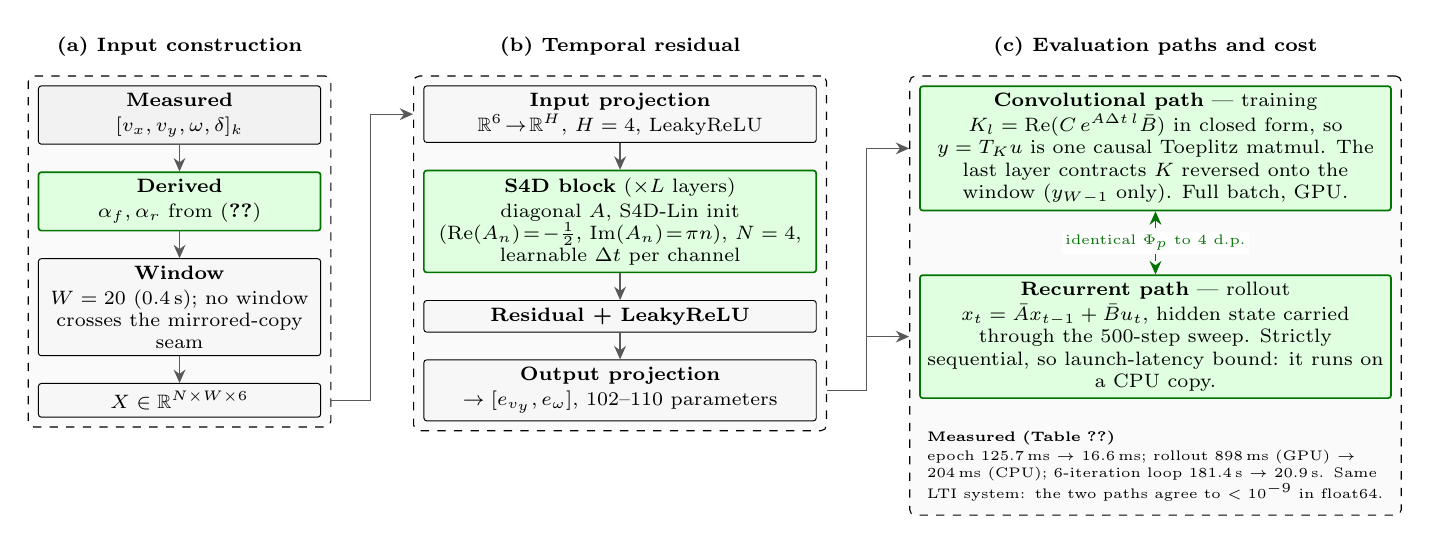
\begin{tikzpicture}[
  font=\scriptsize,
  >={Stealth[length=1.7mm,width=1.5mm]},
  blk/.style     = {draw, rounded corners=1pt, align=flush center, inner sep=2.6pt,
                    text width=#1, fill=white, line width=0.35pt},
  sig/.style     = {blk=34mm, fill=black!5},
  aug/.style     = {blk=34mm, fill=green!12, draw=green!45!black, line width=0.6pt},
  net/.style     = {blk=48mm, fill=black!3},
  ssm/.style     = {blk=48mm, fill=green!12, draw=green!45!black, line width=0.6pt},
  path/.style    = {blk=58mm, fill=white},
  fast/.style    = {path, fill=green!12, draw=green!45!black, line width=0.6pt},
  note/.style    = {font=\tiny, align=left, inner sep=1.6pt, text width=58mm},
  flow/.style    = {->, line width=0.5pt, black!65},
  eq/.style      = {<->, line width=0.6pt, green!45!black, dashed},
  lbl/.style     = {font=\tiny, inner sep=1.2pt, fill=white, midway},
  hdr/.style     = {font=\scriptsize\bfseries, align=center}
]

\def\vgap{3.4mm}

% ======================= (a) input construction ============================
\node[sig, anchor=north west] (raw) at (0,0)
  {\textbf{Measured}\\[1pt] $[v_{x},v_{y},\omega,\delta]_{k}$};
\node[aug, below=\vgap of raw] (slip)
  {\textbf{Derived}\\[1pt] $\alpha_{f},\alpha_{r}$ from \eqref{eq:slip}};
\node[blk=34mm, below=\vgap of slip, fill=black!3] (win)
  {\textbf{Window}\\[1pt] $W=20$ (\SI{0.4}{\second}); no window crosses the
   mirrored-copy seam};
\node[blk=34mm, below=\vgap of win, fill=black!3] (xin)
  {$X\in\mathbb{R}^{N\times W\times 6}$};

\draw[flow] (raw)  -- (slip);
\draw[flow] (slip) -- (win);
\draw[flow] (win)  -- (xin);

\begin{scope}[on background layer]
  \node[draw, dashed, rounded corners=2pt, inner sep=3.4pt, fill=black!2,
        fit=(raw)(slip)(win)(xin)] (panela) {};
\end{scope}
\node[hdr, above=1.2mm of panela.north] {(a) Input construction};

% ========================== (b) S4D residual ===============================
\node[net, right=13mm of raw.north east, anchor=north west] (proj)
  {\textbf{Input projection}\\[1pt] $\mathbb{R}^{6}\!\to\!\mathbb{R}^{H}$,
   $H=4$, LeakyReLU};
\node[ssm, below=\vgap of proj] (s4d)
  {\textbf{S4D block} ($\times L$ layers)\\[1pt]
   diagonal $A$, S4D-Lin init
   ($\mathrm{Re}(A_{n})\!=\!-\tfrac12$, $\mathrm{Im}(A_{n})\!=\!\pi n$),
   $N=4$, learnable $\Delta t$ per channel};
\node[net, below=\vgap of s4d] (res)
  {\textbf{Residual + LeakyReLU}};
\node[net, below=\vgap of res] (out)
  {\textbf{Output projection}\\[1pt] $\to[e_{v_{y}},e_{\omega}]$,
   \num{102}--\num{110} parameters};

\draw[flow] (proj) -- (s4d);
\draw[flow] (s4d)  -- (res);
\draw[flow] (res)  -- (out);

\begin{scope}[on background layer]
  \node[draw, dashed, rounded corners=2pt, inner sep=3.4pt, fill=black!2,
        fit=(proj)(s4d)(res)(out)] (panelb) {};
\end{scope}
\node[hdr, above=1.2mm of panelb.north] {(b) Temporal residual};

% Panel-to-panel link: anchored on the dashed borders and turned inside the
% gap, so it never crosses either box.
\draw[flow] (panela.east|-xin) -- ++(5mm,0) |- (panelb.west|-proj);

% ===================== (c) two evaluation paths ============================
\node[fast, right=13mm of proj.north east, anchor=north west] (conv)
  {\textbf{Convolutional path} --- training\\[1pt]
   $K_{l}=\mathrm{Re}(C\,e^{A\Delta t\,l}\bar B)$ in closed form, so
   $y=T_{K}u$ is one causal Toeplitz matmul. The last layer contracts $K$
   reversed onto the window ($y_{W-1}$ only). Full batch, GPU.};
% 8 mm, not \vgap: the "identical Phi_p" label rides on the arrow between these
% two boxes and needs a gap taller than itself, or it lands on their borders.
\node[fast, below=8mm of conv] (rec)
  {\textbf{Recurrent path} --- rollout\\[1pt]
   $x_{t}=\bar A x_{t-1}+\bar B u_{t}$, hidden state carried through the
   500-step sweep. Strictly sequential, so launch-latency bound: it runs on a
   CPU copy.};
\node[note, below=\vgap of rec] (cost)
  {\textbf{Measured (Table~\ref{tab:runtime})}\\[1pt]
   epoch \SI{125.7}{\milli\second} $\to$ \SI{16.6}{\milli\second};
   rollout \SI{898}{\milli\second} (GPU) $\to$ \SI{204}{\milli\second}
   (CPU); 6-iteration loop \SI{181.4}{\second} $\to$ \SI{20.9}{\second}.
   Same LTI system: the two paths agree to $<10^{-9}$ in float64.};

\draw[eq] (conv) -- node[lbl]{identical $\phip$ to 4 d.p.} (rec);

\begin{scope}[on background layer]
  \node[draw, dashed, rounded corners=2pt, inner sep=3.4pt, fill=black!2,
        fit=(conv)(rec)(cost)] (panelc) {};
\end{scope}
\node[hdr, above=1.2mm of panelc.north] {(c) Evaluation paths and cost};

\draw[flow] (panelb.east|-out) -- ++(5mm,0) |- (panelc.west|-conv);
\draw[flow] (panelb.east|-out) -- ++(5mm,0) |- (panelc.west|-rec);

\end{tikzpicture}
}
\caption{Stage~1 of Fig.~2 of the main paper with the physics-augmented input
vector (Section~\ref{sup:physinputs}) and the S4D temporal residual
(Section~\ref{sup:s4}). Green marks what differs from the baseline MLP
residual. (a) The four measured signals are augmented with the two slip angles
of main-paper (3) and cut into $W=20$ sample windows. (b) The residual stack:
input projection to $H$ channels, S4D blocks with a diagonal state-transition
matrix, and an output projection to $[e_{v_{y}},e_{\omega}]$. (c) The same
linear time-invariant system is evaluated two ways, as a causal convolution
with the closed-form impulse response for training and as a recurrence for
stage~2's stateful rollout, which is what makes the architecture affordable on
a CPU without changing a single identified coefficient
(Section~\ref{sup:s4cost}).}
\label{fig:pipelines4}
\end{figure*}

\subsection{Evaluating the temporal residual at CPU cost}
\label{sup:s4cost}
A temporal residual is only usable on-vehicle if it fits inside the
re-identification period on the hardware the car carries, which is typically a
CPU. Profiled as first written, the S4D path cost \SI{125.7}{\milli\second} per
epoch on a GPU and \SI{898}{\milli\second} per stage-2 rollout, putting a
six-iteration identification at \SI{181.4}{\second}, longer than the
\SI{30}{\second} data window it consumes. Three changes remove that cost
without altering the arithmetic. None is novel as a technique; what matters
here is that the resulting pipeline is real-time-plausible on commodity
hardware, and that the equivalence was verified rather than assumed.

\paragraph{Closed-form kernel instead of a scan}
A diagonal $A$ makes the block's impulse response available in closed form,
\begin{equation}
K_{l}=\mathrm{Re}\big(C\,e^{A\Delta t\,l}\,\bar B\big),\qquad l=0,\dots,W-1,
\label{eq:s4kernel}
\end{equation}
so a length-$W$ window is one Vandermonde product followed by a causal Toeplitz
matrix product, rather than $W$ sequential steps~\cite{gu2022s4d}. At $W=20$
the dense Toeplitz product is cheaper than the FFT convolution of the original
S4~\cite{gu2022s4} and than a parallel associative scan~\cite{smith2023s5};
both are the right choice at sequence lengths orders of magnitude longer than
this one. Because the stack's output layer reads only the window's last
timestep, that layer contracts the reversed kernel straight onto the window and
skips $W-1$ of its outputs. Cost: \SI{125.7}{\milli\second} to
\SI{26.7}{\milli\second} per epoch.

\paragraph{Loop-invariant physics-loss terms}
Under the physics-informed objective, the nominal Pacejka rollout, the mirrored
batch and the constant terms of the symmetry residual depend on the nominal
model only, which is fixed for the whole training call, so they are precomputed
once per call instead of once per epoch. The three forward passes the objective
used to make (data, mirror, smoothness) collapse into one pass over a
double-length batch, with the smoothness Jacobian taken off the same graph.
Cost: \SI{26.7}{\milli\second} to \SI{16.6}{\milli\second} per epoch, with the
loss value unchanged bit for bit.

\paragraph{The rollout belongs on a CPU}
Stage~2 is 500 strictly sequential single-sample steps carrying the S4D hidden
state, each with a host synchronisation. That is pure kernel-launch latency on
a GPU: \SI{898}{\milli\second} on CUDA against \SI{204}{\milli\second} on a CPU
copy of the same weights. The rollout is therefore run on a CPU copy whatever
device training used, following the recurrent path of
Fig.~\ref{fig:pipelines4}(c), and only the full-batch training stays on the
GPU, where it is \num{2.4}$\times$ faster than a CPU. This is the one place where the two evaluation paths of the
same system have to agree exactly, and they are pinned by a regression test to
$<10^{-9}$ in double precision.

End to end this takes a six-iteration identification from \SI{181.4}{\second}
to \SI{20.9}{\second} (\num{8.7}$\times$) on the same synthetic
\SI{30}{\second} lap, with the identified Pacejka coefficients agreeing to four
decimal places (Table~\ref{sup:tabruntime}). We deliberately did \emph{not}
touch the knobs that trade accuracy for speed: epoch count, iteration count,
early stopping, warm-starting the network from the previous iteration's
weights, or dropping the smoothness term. Those change the identified tire and
are a modelling decision, not a free speedup.

\section{Identification Cost, per Phase}
\label{sup:runtime}

\subsection{Identification cost}

Section~\ref{sup:s4cost}'s claim is that the temporal residual is affordable
on the hardware a vehicle carries; Table~\ref{sup:tabruntime} is the measurement,
on a synthetic \SI{30}{\second} lap and the same six co-identification
iterations throughout. The per-stage rows and the end-to-end totals were
measured separately and are not a decomposition of each other: the stage rows
reconstruct \SI{156.2}{\second} of the \SI{181.4}{\second} before and
\SI{21.1}{\second} of the \SI{20.9}{\second} after, so the residual
\SI{25.2}{\second} of fixed cost visible before is not visible after. We
report both as measured rather than reconciling them by attribution. Every
step was verified against the implementation it replaced before being kept: the convolutional and recurrent paths of
Fig.~\ref{fig:pipelines4}(c) agree to $<10^{-9}$ in double precision (pinned by
a regression test), the rewritten physics-informed loss is bit-identical, and
the full six-iteration loop lands on the same Pacejka coefficients to four
decimal places, the remaining difference being float32 reordering over
\num{1200} optimiser steps.

\begin{table}[t]
\caption{Cost of one S4D identification on a synthetic \SI{30}{\second} lap.}
\label{sup:tabruntime}
\centering
\begin{threeparttable}
\scriptsize
\begin{tabular}{@{}p{3.1cm}ccc@{}}
\toprule
Stage & Device & Before & After\\
\midrule
Training epoch: scan $\to$ kernel \eqref{eq:s4kernel} & GPU &
\SI{125.7}{\milli\second} & \SI{26.7}{\milli\second}\\
Training epoch: physics-loss hoist and fusion & GPU &
\SI{26.7}{\milli\second} & \SI{16.6}{\milli\second}\\
Stage-2 rollout, 500 sequential steps & GPU $\to$ CPU &
\SI{898}{\milli\second} & \SI{204}{\milli\second}\\
\addlinespace
Identification, 6 iterations & mixed & \SI{181.4}{\second} &
\SI{20.9}{\second}\\
\bottomrule
\end{tabular}
\begin{tablenotes}[flushleft]\scriptsize
\item The optimisations are exact: no epoch count, iteration count, early-stopping rule or loss weight was changed, and the identified coefficients agree to four decimal places.
\item The first three rows are per-stage micro-benchmarks of the named stage;
the last row is a separate end-to-end measurement of the whole six-iteration
loop and includes everything the micro-benchmarks exclude: data preparation,
the per-iteration network re-initialisation and the six Pacejka fits.
\item The two therefore do not sum: at \num{1200} epochs and six rollouts the stage rows account for \SI{156.2}{\second} of the \SI{181.4}{\second} before and \SI{21.1}{\second} of the \SI{20.9}{\second} after. The \num{8.7}$\times$ is the ratio of the two end-to-end measurements.
\end{tablenotes}
\end{threeparttable}
\end{table}

Two consequences follow. At \SI{20.9}{\second} the identification fits inside
the \SI{30}{\second} re-identification period of
Section~V-F of the main paper, so the temporal residual is a deployable
option rather than an offline one; at \SI{181.4}{\second} it was not. And the
device split is not incidental: the stage-2 rollout is strictly sequential and
single-sample, so it is \num{4.4}$\times$ \emph{faster} on a CPU, while
full-batch training over $\approx\num{3000}$ windows remains
\num{2.4}$\times$ faster on the GPU. A pipeline pinned to one device pays one
of those two penalties.

\section{The Baseline Pipeline Against This Work}
\label{sup:baseline}

\subsection{Baseline pipeline versus this work}
\label{sup:baselinecmp}

Table~\ref{sup:tabbaseline} places the pipeline as published~\cite{ontrack2025}
beside the pipeline as it stands here, on the axes that changed. The residual
model, the data budget, the four-stage loop and the steady-state force recovery
are inherited unchanged; what differs is the configuration of the virtual-data
step, the regularisation topology, the measurement chain, and the contract at
the output. Table~III of the main paper's comparison is a subset of these axes:
the rollout correction of Section~V-B of the main paper is active in both
runs of Section~VI-C of the main paper, so that section measures the remaining
four settings and not the rollout.

\begin{table}[t]
\caption{The baseline pipeline~\cite{ontrack2025} against this work, on the
axes that differ.}
\label{sup:tabbaseline}
\centering
\begin{threeparttable}
\scriptsize
\setlength{\tabcolsep}{3pt}
\begin{tabular}{@{}p{1.95cm}p{2.55cm}p{3.0cm}@{}}
\toprule
Axis & Baseline~\cite{ontrack2025} & This work\\
\midrule
Platform & 1:10, \SI{3.7}{\kilo\gram}, $L=\SI{0.32}{\meter}$ &
Full scale, \SI{269.6}{\kilo\gram}, $L=\SI{1.53}{\meter}$\\
Rollout speed & $\mathrm{clip}(\overline{v_{x}},2,4)\,\si{\meter\per\second}$ &
From the measured lap, floored at \SI{15}{\meter\per\second}\\
Reachable $\mu$ & $\approx2.0$ (adequate) & $0.43$ under the baseline clip;
$\ge1.2$ after correction\\
Sweep amplitude & Fixed \SI{0.4}{\radian} &
$1.5P_{99}(|\delta_{\mathrm{obs}}|)$, clipped to
$[\delta_{\min},\delta_{\max}]$\\
Regularisation & None; each fit is the next start point &
Tikhonov to a \emph{frozen} prior; start point still tracks\\
Steering signal & Command & Achieved road-wheel angle\\
Mass, geometry & Configuration file & Measured static wheel loads\\
Friction prior & --- & Per-axle brush fit of $(C_{\alpha},\mu)$ from IMU and
odometry, gated; $P_{99}$ of $|a|/g$ as fallback; always a floor\\
Solver & Trust-region, single start & Multi-start, plus simplex and global
options\\
Output contract & Per-coefficient box constraints & Gates on derived
quantities at the controller interface\\
Residual objective & One-step MSE & MSE plus quasi-steady balance, left/right
symmetry and input-gradient penalties, \eqref{eq:pinnloss}\\
Residual inputs & State, command & \emph{inherited} plus axle slip angles
(Sec.~\ref{sup:physinputs})\\
Residual model & MLP, 58 parameters & \emph{inherited} as default; S4D
temporal residual shipped\\
Residual cost & Not reported & S4D identification \SI{181.4}{\second}
$\rightarrow$ \SI{20.9}{\second}, exact (Table~\ref{sup:tabruntime})\\
Data budget & \SI{30}{\second}, one controller-free lap & \emph{inherited}\\
Force recovery & Quasi-steady yaw balance & \emph{inherited}\\
Ground truth & Steady-state manoeuvre in a large space &
Simulator per-wheel force, slip and load\\
\bottomrule
\end{tabular}
\begin{tablenotes}[flushleft]\scriptsize
\item Rows marked \emph{inherited} are unchanged and are listed so that the
extent of the modification is unambiguous.
\end{tablenotes}
\end{threeparttable}
\end{table}

\section{Supporting Result Figures}
\label{sup:figs}

These figures accompany Section~VI of the main paper; every metric they show is
also in its cross-run comparison table.

\begin{figure}[t]
\centering

\includegraphics[width=\columnwidth]{mu_error_by_scenario}
\caption{Peak-friction error per axle against the effective coefficient the
simulator reports per wheel ($\mu=1.05$, static for both runs). The corrected
configuration's error is an order of magnitude smaller on both axles
(\num{0.041} and \num{0.048} against \num{0.762} and \num{0.772} RMSE); the
inherited configuration's error is not a mis-estimate but a coefficient parked
on its upper bound.}
\label{fig:muerror}
\end{figure}


\begin{figure}[t]
\centering

\includegraphics[width=\columnwidth]{tire_force_rmse_by_scenario}\\[2pt]

\includegraphics[width=\columnwidth]{tire_force_r2_by_scenario}
\caption{Axle lateral force against the plant's per-wheel telemetry, per axle:
RMSE (top) and $R^{2}$ (bottom). The ordering reverses between axles, and this
is the one family of metrics on which the inherited configuration is better:
at the \SI{2.2}{\degree} of slip the lap reaches, a slope deficit costs force
and a wrong peak factor costs nothing.}
\label{fig:forcebars}
\end{figure}


\begin{figure*}[t]
\centering

\includegraphics[width=\textwidth]{tire_force_error_hist_by_scenario}
\caption{Distribution of the axle lateral-force error (truth minus estimate),
shared bin edges over the pooled central \SI{99}{\percent} and normalised to
the sample count of each run. Both are centred; the inherited configuration
buys its lower front RMSE with the heavier tail (maximum absolute error
\SI{215}{\newton} against \SI{138}{\newton} front, \SI{223}{\newton} against
\SI{85}{\newton} rear).}
\label{fig:forcehist}
\end{figure*}


\begin{figure*}[t]
\centering

\includegraphics[width=\textwidth]{tire_force_timeseries_by_scenario}
\caption{Axle lateral force over the run, one row per configuration. The two
runs are separate laps and share only $t=0$, so each estimate is drawn against
its own ground truth. Where the force is largest each model errs in the
direction its initial slope predicts, the corrected configuration short and
the inherited one long.}
\label{fig:forcetime}
\end{figure*}


\begin{figure}[t]
\centering

\includegraphics[width=\columnwidth]{state_rmse_by_scenario}
\caption{One-step prediction RMSE for $v_{y}$ and $\omega$ against the
persistence baseline of the same run. Neither identified model beats
persistence at the \SI{0.035}{\second} model step.}
\label{fig:staterms}
\end{figure}


\begin{figure}[t]
\centering

\includegraphics[width=\columnwidth]{state_error_hist_v_y}
\caption{Lateral-velocity prediction error (truth minus estimate). The two
configurations are indistinguishable on this channel
(\SI{0.027}{\meter\per\second} against \SI{0.022}{\meter\per\second} RMSE);
the yaw channel, not this one, is where they differ.}
\label{fig:statehistvy}
\end{figure}


\begin{figure}[t]
\centering

\includegraphics[width=\columnwidth]{state_error_hist_omega}
\caption{Yaw-rate prediction error (truth minus estimate). The difference
between the configurations is tail mass, not centre.}
\label{fig:statehistomega}
\end{figure}


\begin{figure*}[t]
\centering

\includegraphics[width=\textwidth]{state_timeseries_by_scenario}
\caption{Estimated states against truth over the run, one row per
configuration, \SI{591}{\second} and \SI{564}{\second} of driving. At
this compression the traces overlie their ground truth almost everywhere,
which is the point: a one-step metric on a smooth racing line is close to
uninformative, and the visible departures are the yaw-rate excursions that
separate the two configurations in Fig.~\ref{fig:statehistomega}.}
\label{fig:statetime}
\end{figure*}


\begin{figure}[t]
\centering

\includegraphics[width=\columnwidth]{e_y_error_hist_by_scenario}
\caption{Signed lateral tracking error over the whole run. The corrected
configuration's distribution is narrower about a comparable centre, at sample
standard deviation \SI{0.279}{\meter} against \SI{0.301}{\meter} and mean
\SI{0.014}{\meter} against \SI{0.039}{\meter}, so the improvement is in
spread, not in bias.}
\label{fig:eyhist}
\end{figure}


\begin{figure}[t]
\centering

\includegraphics[width=\columnwidth]{itae_by_scenario}
\caption{ITAE of the lateral error, overall and split by the active
controller. The pure-pursuit phase is ordered the other way and is two orders
of magnitude smaller.}
\label{fig:itae}
\end{figure}


\bibliographystyle{IEEEtran}
\bibliography{references}

\end{document}
